\chapter{Introduction}
\label{chap:intro}

Embedded systems are widely used today in various applications, from cars, cell phones, home automation, to critical infrastructures
like power plants and power grids, water, gas or electricity distribution systems and production systems for food and other products.

Since they were almost isolated from the network, embedded systems have not been designed and built with security concepts in mind.
However, many recent cyber-attacks demonstrated that such an assumption is no more valid, and the security of embedded systems became an open question to deal with.

Unfortunately, this could be a more challenging problem with respect to security for desktop and enterprise computing, for the following reasons:
\begin{itemize}[itemsep=2pt,topsep=0pt]
	\item the limited capabilities and the strict timing requirements these systems have;
	\item the physical side effects a security breach may lead to, \eg property damage, personal injury, death and even environmental or nuclear disaster.
\end{itemize}

In the next sections we first describe a particular type of embedded systems, then present the problem on which the rest of the paper is focused,
and define the goal of this thesis.


\section{Programmable Logic Controllers}

Within the context of an Industrial Control System (ICS), embedded systems are better known as Programmable Logic Controllers (PLCs).
PLCs are special-purpose embedded systems, usually deployed into harsh environments to control critical processes,
\eg automotive systems, assembly lines, robotic devices or any industrial machine that requires high control precision and reliability.

A simplified version of the environment in which a PLC may operate is outlined in \myfig{fig:plc-env}.
\begin{figure}[h]
\centerline{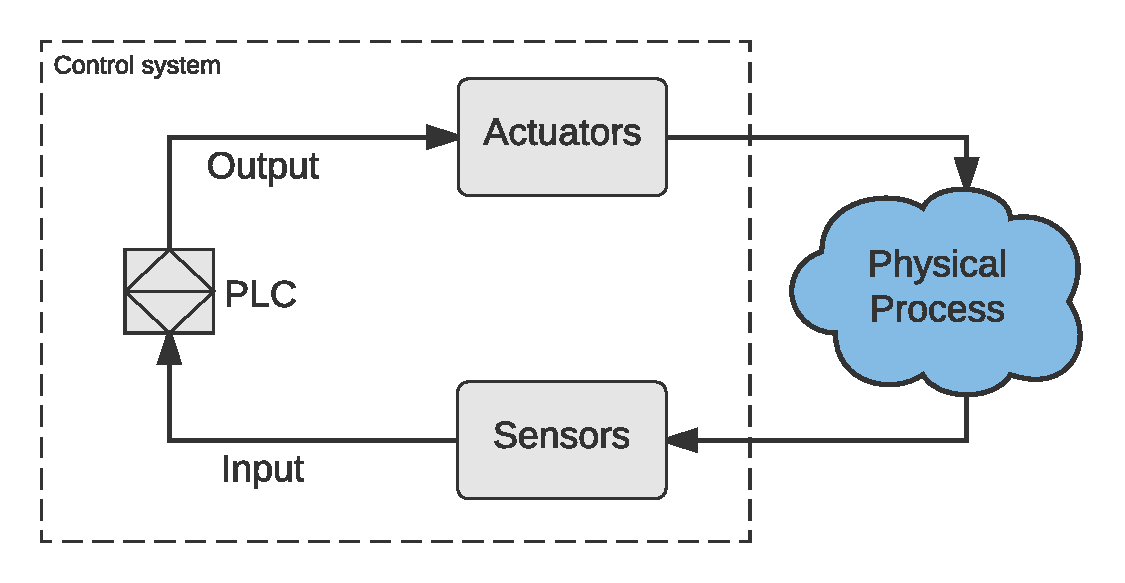
\includegraphics[width=0.6\textwidth]{res/plc-env}}
\caption{PLC environment\label{fig:plc-env}}
\end{figure}

The PLC interacts with the physical world through external components called \emph{sensors} and \emph{actuators}.
The sensors are responsible for reporting measurements about a set of properties of the physical process,
while the actuators, as the name suggests, act on the process modifying its current state.

The main task of a PLC is contained into the control program (the \emph{PLC logic}) which is programmed and loaded by an industrial operator.
The logic is executed repeatedly as long as the controlled system is running. Each single execution is known as \emph{PLC scan cycle}.
For each scan cycle, the PLC reads the current state of the physical process measured by sensors.
Internally, the logic takes these values as input and performs some calculations based on the loaded control algorithm.
The output of the logic is then sent to the actuators, thus modifying the state of the controlled process.

The PLC main scan cycle is shown in \myfig{fig:scan-cycle}.
\begin{figure}[h]
\centerline{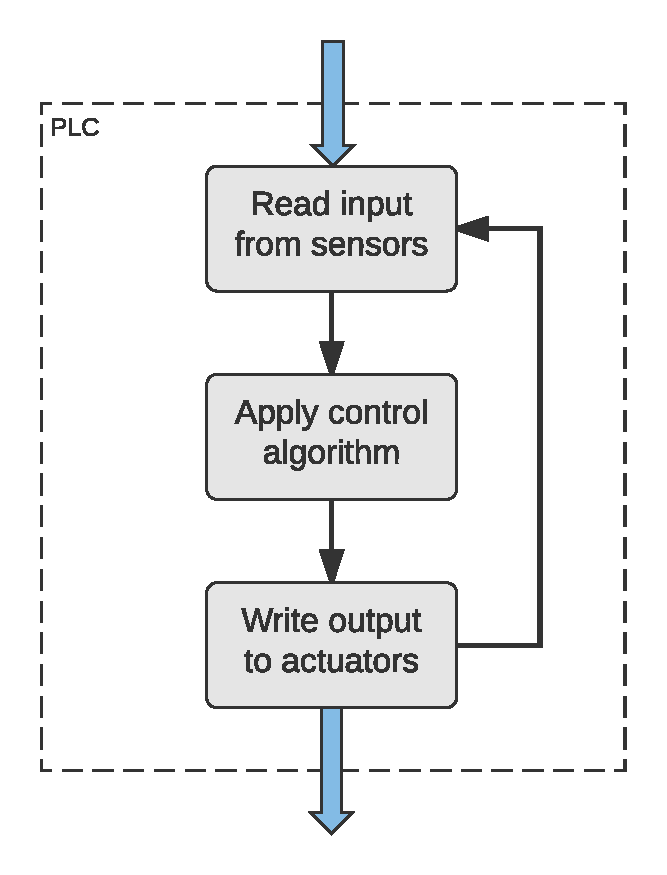
\includegraphics[width=0.4\textwidth]{res/scan-cycle}}
\caption{PLC logic main scan cycle\label{fig:scan-cycle}}
\end{figure}

Based on the nature of the controlled process, the logic must satisfy different safety and timing properties.
Furthermore, the majority of the PLCs are provided with a real-time operating system, in order to guarantee that the strict timing requirements are always respected.
A violation of these requirements may lead to an unsafe behaviour of the physical process, and the consequences are heavily related to the nature of the process under control.


\section{Problem statement}

From a computer engineering perspective, PLCs control the outside world via their Input/Output (I/O) interfaces (or I/O \emph{pins}).
Therefore, it is crucial that these interfaces are both reliable and secure. They are accessible through specific registers within a particular memory region of the system,
called I/O memory. By accessing I/O memory, I/O interfaces can be configured in several different ways, according to the desired behaviour.
On almost every system, it is possible to change this configuration while the system is running.
This feature is managed by a subsystem called \emph{pin controller}, and the registers used for this purpose are known as \emph{pin control registers}.

The problem here relies on the fact that there is neither any memory protection mechanism nor any hardware interrupt designed for restricting the access
to the addresses of these registers. They can be easily written by a malicious application even while the system is active, over-writing the current hardware configuration.
Therefore, a malicious user, can manipulate I/O configuration at his will, modifying the behaviour of I/O interfaces.
Hence, the interaction with the physical process may be altered in a dramatic way.
In \cite{ghostplc}, Abbasi et al. showed how this feature is actually exploitable by attackers, who can tamper with
the integrity or the availability of legitimate I/O operations of PLCs, factually changing the way they interact with sensors and actuators.
Based on these observations, they introduced a novel attack technique against PLCs, which they call \emph{Pin Control Attack}, or \emph{I/O attack} \cite{tech-ghostplc}.
In the rest of the paper, we use these two names interchangeably, although the former strictly refers to pin control registers, while the latter
might be used to refer to a wider range of attacks, by extending the target to any other I/O register that could affect PLC operations
(\eg devices' registers, interrupt registers, etc.). The salient features of this new class of attacks are:
\begin{enumerate}[itemsep=2pt,topsep=0pt]
	\item \itemname{Stealthiness}: the alteration of I/O configuration does not generate any interrupt signal, preventing the Operating System (OS) to react to it.
		Moreover, it is entirely different in execution from traditional techniques typically monitored by off-the-shelf protection systems
		(\eg manipulation of kernel structures or system call hooking).
	\item \itemname{Low-level target}: the attack is not directed to the firmware, nor the PLC runtime/logic, as typical state-of-the-art attacks do.
		Here the attacker, instead, aims to lower level resources of the system, such as the I/O hardware configuration.
	\item \itemname{Viability}: as demonstrated in \mychap{chap:attack}, it is possible to build concrete attack using it.
\end{enumerate}
To better understand a possible attack scenario, \myfig{fig:control} shows a simplified control system.
\begin{figure}[h!]
\centerline{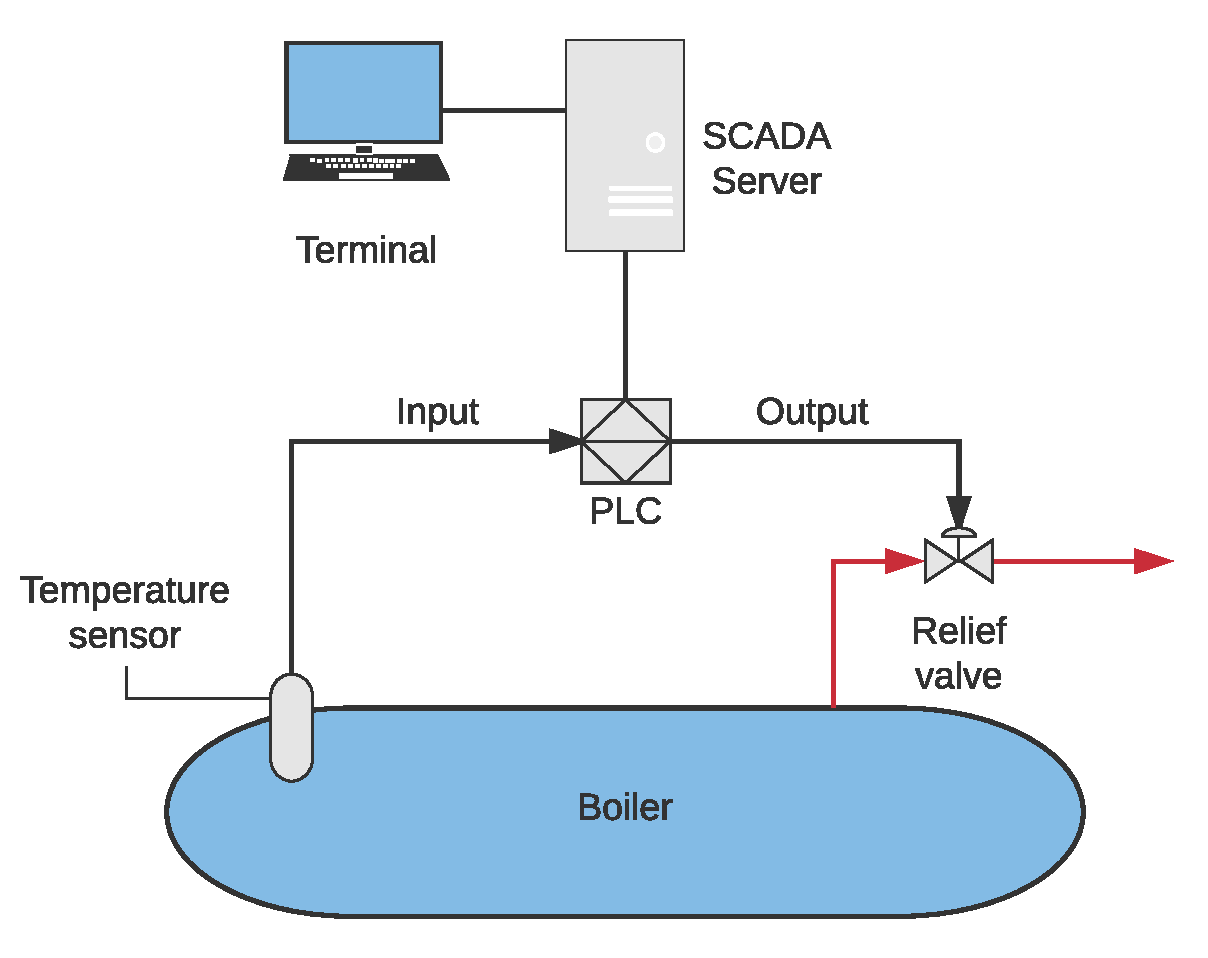
\includegraphics[width=0.6\textwidth]{res/control}}
\caption{Simplified control system: a possible target of Pin Control Attack.\label{fig:control}}
\end{figure}

The system consists of a boiler equipped with a relief valve driven by the PLC according to the value provided by a temperature sensor.
The PLC is connected to a SCADA server (Supervisory Control And Data Acquisition) to keep trace of its operation.
The server is accessible from a terminal, through which an operator can load the logic into the PLC and monitor its current state.

Suppose that the PLC logic is programmed to read the values from the temperature sensor, and to open the relief valve if the temperature goes over $80^\circ C$.
An attacker could tamper the temperature value read by the PLC, re-configuring the I/O interface related to the sensor as output and writing its own desired value
(\eg always $\SI{50}{\degree C}$) regardless of the actual temperature.
Even simpler, one could reconfigure the I/O pin connected to the valve (\eg setting it as input) factually disabling any eventual command to the actuator.

Actually there is no detection mechanism able to react to these configuration changes, neither in the PLC firmware nor in the control system.
Moreover, the operator of the control system will not be able to see the real temperature nor the actual valve state from the terminal,
so it may likely not notice the intrusion at all.
Such a condition may lead to an uncontrolled overheating, and if it is not detected in time it could even make the boiler to explode.


\section{Aim of the thesis}

The goal of this thesis is to analyse the threat, design and implement a detection system for I/O Attack.
It is a challenging task for at least two reasons:
\begin{enumerate}
	\item The system lacks hardware interrupts, so it is not possible to directly react to any configuration change. More complex detection mechanisms are needed
		in order to achieve the highest possible detection rate.
	\item The resources available within an embedded system like a PLC are extremely limited. Therefore, our solution must be extremely agile and light,
		since the smallest delay in the PLC I/O operation may have unintended consequences for the controlled process.
\end{enumerate}

The work has been divided into three main steps.
First, we discuss the idea behind the attack, describe its threat model and its different implementations on an Embedded Linux ARM-based architecture.
We also analyse and experiment the feasibility of the attack on a real PLC.
Second, based on the assumptions contained in the threat model and on the findings of our analysis, we describe the design and the implementation of our defense.
The target of our implementation is a non real-time version of the Linux kernel running on an ARM-based System on Chip,
as this is one of the solutions actually used for mid-range embedded systems as PLCs.
Finally, we validate the proposed solution with respect to the following parameters: detection rate and performance overhead.
A brief organisation of the rest of the thesis follows in the next section.


\section{Organisation}

In \mychap{chap:related} we list the known attacks to embedded systems existing in the literature, and then discuss the off-the-shelf protection mechanisms.
To the best of our knowledge at the time of writing, as I/O Attack is a new kind of attack, none of the existing protections is able to prevent nor detect it.
\mychap{chap:attack} contains, after a brief description of the embedded systems architecture, a detailed analysis of the attack design and implementation.
In \mychap{chap:defense} we present the architecture of our proposed detection mechanism, and describe the implementation in detail.
The \mychap{chap:results} provides the results obtained during the experiments, showing the detection rate and the performance overhead on a PLC environment.
Finally, in \mychap{chap:conclusions} we analyse the shortcomings of our defense and the possible future works and improvements.
